\documentclass[xcolor=pdftex,dvipsnames]{beamer}
\usefonttheme{structurebold}

%\usetheme{default}
%\usetheme{Warsaw}
%\usetheme{Copenhagen}
%\usetheme{Berlin}
%\usetheme{Frankfurt}
\usetheme{CambridgeUS}
\usepackage{tikz}
\usetikzlibrary{positioning}
\usepackage{graphics}
\usepackage{kotex}
\usepackage{url}
\usepackage{multirow,array}
\setbeamertemplate{footline}[page number]{}

\title[]{현대비교정부론}
\author[]{강명세}
\institute[]{세종연구소}
\date[]{3주차}

\begin{document}

\begin{frame}
\titlepage
\transboxout
\end{frame}


\begin{frame}
\frametitle{Outline}
\begin{itemize}
\item What is Politics?
\item Game Theory
\item Exit, Voice, and Loyalty Game
\end{itemize}
\end{frame}

\section{정치란 무엇인가?}

\begin{frame}
\frametitle{정치}
\begin{itemize}
\item Politics is the subset of human behavior that involves the use of \emph{power} or influence
\item Power is involved whenever individuals cannot accomplish their goals without:
\begin{itemize}
\item either trying to influence the behavior of others
\item or trying to wrestle free from the influence exerted by others
\end{itemize}
\end{itemize}
\end{frame}

\begin{frame}
\frametitle{Exit, Voice, and Loyalty}
\begin{itemize}
\item Albert Hirschman (1970), \emph{Exit, Voice, and Loyalty: Responses to Decline in Firms, Organizations, and States}
\item In our exercise, we will focus on the power relationship between citizens and the state.
\begin{itemize}
\item when citizens will take direct actions against the state
\item when the state will respond positively to the demands of citizens
\item when the state will ignore citizens
\end{itemize}
\item Suppose that there has been some change in your environment that you do not like $\rightarrow$ What would you do about it?
\end{itemize}
\end{frame}

\begin{frame}
\frametitle{Exit, Voice, and Loyalty}
\begin{itemize}
\item Three possible responses:
\begin{itemize}
\item \underline{Exit}: You accept that there has been a deleterious change in your environment and you alter your behavior to achieve the best outcome possible given your new environment
\item \underline{Voice}: You use your voice (complain, protest, lobby, or direct action) to try to change the environment back to its original condition
\item \underline{Loyalty}: You accept that your environment has changed and make no change to your behavior
\end{itemize}
\item How should the citizens respond?
\begin{itemize}
\item Citizen's choice will \emph{depend} on what she expects to happen when she chooses one of these options
\item To know what to do, she needs to know what the state would do if she used one of these options
\end{itemize}
\end{itemize}
\end{frame}

\begin{frame}
\frametitle{Exit, Voice, and Loyalty}
\end{frame}


\section{게임이론}

\begin{frame}
\frametitle{게임이론}
\begin{itemize}
\item 정치는 전략적 상호작용의 결과
행위자 Players = {1, 2} \\
전략1 = {거부, 협조}, 전략2={거부,협조}\\

\

\item \underline{전략적 상황}\\
각각의 선택이 결과(payoff)를 결정\\
전략 : 모든 가능한 조건에 대비한 선택의 집합 \\

\end{itemize}
\end{frame}


\begin{frame}
\frametitle{게임이론}
\begin{itemize}
\item 정상게임 / 전략게임
\begin{itemize}
\item 수혜의 집합
\item 동시결정
\end{itemize}
\item 확장형 게임 
\begin{itemize}
\item 게임나무
\item 순차적 선택
\end{itemize}
\end{itemize}
\end{frame}

\begin{frame}
\frametitle{Prisoner's Dilemma game}
\begin{itemize}
\item 두 임원 구속
\item 검사 전략

\begin{enumerate}
\item ``모두 거부하면, 경범죄"
\item ``모두 자백하면, 모두 유죄"
\item ``혼자 협조하면, 감형"
\item ``혼자만 거부하면, 중형"
\end{enumerate}

\end{itemize}
\end{frame}

\begin{frame}
\frametitle{PD game}
\begin{figure}
\begin{center}
  \includegraphics[width=0.75\textwidth]{PD.png}\\
\end{center}
\end{figure}
\end{frame}

\begin{frame}
\frametitle{PD game - Nash Equilibrium}
\begin{figure}
\begin{center}
  \includegraphics[width=0.75\textwidth]{PD_Nash.png}\\
\end{center}
\end{figure}
\end{frame}

\begin{frame}
\frametitle{Solution concept : Nash Equilibrium} 
\begin{itemize}
\item Solution concept for normal form (strategic form) game
\item Nash EQ : A set of strategies in a game such that no player has an incentive to unilaterally change her mind given what the other players are doing
\item Players choose to do what they believe is in their best interest
\item Best responses to each other
\item 영화 \emph{Beaufiful Mind}의 맥주집 장면
\end{itemize}
\end{frame}

\begin{frame}
\frametitle{Chicken game}
\begin{figure}
\begin{center}
  \includegraphics[width=0.75\textwidth]{Chicken.png}\\
\end{center}
\end{figure}
\end{frame}

\begin{frame}{검사전략}
  \begin{table}
    \setlength{\extrarowheight}{3pt}
    \begin{tabular}{cc|c|c|}
      & \multicolumn{1}{c}{} & \multicolumn{2}{c}{임원 $2$}\\
      & \multicolumn{1}{c}{} & \multicolumn{1}{c}{$Refuse$}  & \multicolumn{1}{c}{$Talk$} \\\cline{3-4}
      \multirow{2}*{임원 $1$}  & $Refuse$ & $(-1, -1)$ & $(-10, 0)$ \\\cline{3-4}
      & $Talk$ & $(0, -10)$ & $(-6, -6)$ \\\cline{3-4}
    \end{tabular}
  \end{table}
\end{frame}

\begin{frame}{마피아문화}
  \begin{table}
    \setlength{\extrarowheight}{3pt}
    \begin{tabular}{cc|c|c|}
      & \multicolumn{1}{c}{} & \multicolumn{2}{c}{임원 $2$}\\
      & \multicolumn{1}{c}{} & \multicolumn{1}{c}{$Refuse$}  & \multicolumn{1}{c}{$Talk$} \\\cline{3-4}
      \multirow{2}*{임원 $1$}  & $Refuse$ & $(-1, -1)$ & $(-10,-6)$ \\\cline{3-4}
      & $Talk$ & $(-6, -10)$ & $(-12, -12)$ \\\cline{3-4}
    \end{tabular}
  \end{table}
\end{frame}

\begin{frame}{의리}
  \begin{table}
    \setlength{\extrarowheight}{3pt}
    \begin{tabular}{cc|c|c|}
      & \multicolumn{1}{c}{} & \multicolumn{2}{c}{임원 $2$}\\
      & \multicolumn{1}{c}{} & \multicolumn{1}{c}{$Refuse$}  & \multicolumn{1}{c}{$Talk$} \\\cline{3-4}
      \multirow{2}*{임원 $1$}  & $Refuse$ & $(4, 4)$ & $(-5, 0)$ \\\cline{3-4}
      & $Talk$ & $(0, -5)$ & $(-6, -6)$ \\\cline{3-4}
    \end{tabular}
  \end{table}
\end{frame}

\begin{frame}{Battle of Sex}
  \begin{table}
    \setlength{\extrarowheight}{3pt}
    \begin{tabular}{cc|c|c|}
      & \multicolumn{1}{c}{} & \multicolumn{2}{c}{여자}\\
      & \multicolumn{1}{c}{} & \multicolumn{1}{c}{$Refuse$}  & \multicolumn{1}{c}{$Talk$} \\\cline{3-4}
      \multirow{2}*{남자}  & $Refuse$ & $(2, 1)$ & $(0, 0)$ \\\cline{3-4}
      & $Talk$ & $(0, 0)$ & $(1, 2)$ \\\cline{3-4}
    \end{tabular}
  \end{table}
\end{frame}

\begin{frame}{확장형게임}
\begin{figure}
 	\begin{center}
    \small
    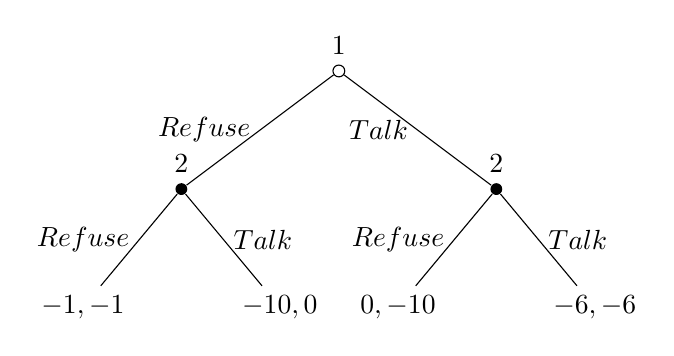
\begin{tikzpicture}[thin,
      level 1/.style={sibling distance=40mm},
      level 2/.style={sibling distance=25mm},
      %level 3/.style={sibling distance=15mm},
      every circle node/.style={minimum size=1.5mm,inner sep=0mm}]
      
      \node[circle,draw,label=above:$1$] (root) {}
        child { node [circle,fill,label=above:$2$] {}
          child { 
            node {$-1,  -1$}
            edge from parent
              node[left] {$Refuse$}}
          child { 
            node {$-10, 0$}
            edge from parent
              node[right] {$Talk$}}
          edge from parent
            node[left] {$Refuse$}}
        child { node [circle,fill,label=above:$2$] {}
          child { 
            node {$0, -10$}
            edge from parent
              node[left] {$Refuse$}}
          child { 
            node {$-6, -6$}
            edge from parent
              node[right] {$Talk$}}
          edge from parent
            node[left] {$Talk$}};

    \end{tikzpicture}
    \end{center}
    \caption{임원의 딜레마}
\end{figure}
\end{frame}

\section{EVL Game}

\begin{frame}
\frametitle{EVL game}
\begin{figure}
\begin{center}
  \includegraphics[width=0.8\textwidth]{EVL_1.png}\\
\end{center}
\end{figure}
\end{frame}

\begin{frame}
\frametitle{EVL game - payoffs}
How much each player values different possible outcomes \\

\begin{tabular}{c c c}
\hline \hline
                  &  Citizen & State \\ 
\hline
Outcome 1 & E & 1 \\ 
Outcome 2 & 0 & 1+L     \\
Outcome 3 & 1-c  & L        \\
Outcome 4 & 0-c & 1+L \\
Outcome 5 & E-c & 1 \\
\hline 
\end{tabular}

\begin{itemize}
\item E: the attractiveness of exit option
\item L: legitimacy
\item c: costs of voice 
\end{itemize}  
\end{frame}

\begin{frame}
\frametitle{EVL game}
\begin{figure}
\begin{center}
  \includegraphics[width=0.8\textwidth]{EVL_2.png}\\
\end{center}
\end{figure}
\end{frame}

\begin{frame}
\frametitle{Solution concept: extensive form game}
\begin{itemize}
\item Subgame Perfect Nash Equilibrium (SPNE)
\begin{itemize}
\item A set of strategies such that each player is playing a Nash Eq. in every subgame
\end{itemize}
\item Backward Induction
\begin{itemize}
\item The process of reasoning backward, from the end of a game to the beginning, to determine an optimal course of action
\end{itemize}
\end{itemize}
\end{frame}


\begin{frame}
\frametitle{EVL game - Case 1}
Case 1: the citizen has a credible exit threat (E$>$0) and state is dependent (L$>$1)
\begin{figure}
\begin{center}
  \includegraphics[width=0.7\textwidth]{EVL_3.png}\\
\end{center}
\end{figure}
\end{frame}

\begin{frame}
\frametitle{EVL game - Case 1}
Case 1: the citizen has a credible exit threat (E$>$0) and state is dependent (L$>$1)
\begin{figure}
\begin{center}
  \includegraphics[width=0.7\textwidth]{Solving_EVL_3.png}\\
\end{center}
\end{figure}
\end{frame}

\begin{frame}
\frametitle{EVL game - Case 1}
Case 1: the citizen has a credible exit threat (E$>$0) and state is dependent (L$>$1)
\begin{itemize}
\item Expected outcome of the game? (Voice, Respond)
\item Payoffs each player receives? (1-c ; L)
\item The equilibrium of the game? (Voice, Exit; Respond)
\begin{itemize}
\item Whay did the state choose to respond positively? Because the state anticipates that the citizen will choose to exit if it did not respond positively
\item The anticipated events can have a tremendous impact on people's behavior even though they might never actually occur
\item The anticipated events never occur precisely because people anticipate them and change their behavior to avoid them
\end{itemize}
\end{itemize}
\end{frame}


\begin{frame}
\frametitle{EVL game - Case 2}
Case 2: the citizen does not have a credible exit threat (E$<$0) and state is dependent (L$>$1)
\begin{figure}
\begin{center}
  \includegraphics[width=0.7\textwidth]{Solving_EVL_4.png}\\
\end{center}
\end{figure}
\end{frame}

\begin{frame}
\frametitle{EVL game - Case 2}
Case 2: the citizen does not have a credible exit threat (E$<$0) and state is dependent (L$>$1)
\begin{itemize}
\item Expected outcome of the game? (Loyalty)
\item Payoffs each player receives? (0 ; 1+L)
\item The equilibrium of the game? (Loyalty, Loyalty; Ignore)
\end{itemize}
\end{frame}


\begin{frame}
\frametitle{EVL game - Case 3}
Case 3: the citizen has a credible exit threat (E$>$0) and state is autonomous (L$<$1)
\begin{figure}
\begin{center}
  \includegraphics[width=0.7\textwidth]{Solving_EVL_5.png}\\
\end{center}
\end{figure}
\end{frame}

\begin{frame}
\frametitle{EVL game - Case 3}
Case 3: the citizen has a credible exit threat (E$>$0) and state is autonomous (L$<$1)
\begin{itemize}
\item Expected outcome of the game? (Exit)
\item Payoffs each player receives? (E ; 1)
\item The equilibrium of the game? (Exit, Exit ; Ignore)
\end{itemize}
\end{frame}


\begin{frame}
\frametitle{EVL game - Case 4}
Case 4: the citizen does not have a credible exit threat (E$<$0) and state is autonomous (L$<$1)
\begin{figure}
\begin{center}
  \includegraphics[width=0.7\textwidth]{Solving_EVL_6.png}\\
\end{center}
\end{figure}
\end{frame}

\begin{frame}
\frametitle{EVL game - Case 4}
Case 4: the citizen does not have a credible exit threat (E$<$0) and state is autonomous (L$<$1)
\begin{itemize}
\item Expected outcome of the game? (Loyalty)
\item Payoffs each player receives? (0 ; 1+L)
\item The equilibrium of the game? (Loyalty, Loyalty ; Ignore)
\end{itemize}
\end{frame}

\begin{frame}
\frametitle{EVL game - Summary}
\begin{figure}
\begin{center}
  \includegraphics[width=1.0\textwidth]{EVL_summary.png}\\
\end{center}
\end{figure}
\end{frame}

\begin{frame}
\frametitle{EVL game - Remarks}
\begin{itemize}
\item The state responds only when the two conditions are met:
\begin{itemize}
\item The citizen must have a credible exit threat ($E>0$)
\item The state must be dependent ($L>1$)
\item E.g., you and your firm
\end{itemize}
\end{itemize}
\end{frame}

\begin{frame}
\frametitle{EVL game - Remarks}
\begin{itemize}
\item In the absence of a credible exit threat ($E<0$), the citizen is a sitting duck
\begin{itemize}
\item African-Americans and Democratic Party 
\item 호남유권자와 민주당
\item Credible exit option is a necessary condition to make sure we are not exploited
\end{itemize}
\end{itemize}
\end{frame}

\begin{frame}
\frametitle{EVL game - Remarks}
\begin{itemize}
\item It is often difficult to learn from observing real-world political situations
\begin{itemize}
\item Citizens do not make a voice. Why? 
\item Not because they are happy
\item But because they expect it is not effective
\end{itemize}
\end{itemize}
\end{frame}

\begin{frame}
\frametitle{EVL game - Remarks}
\begin{itemize}
\item Those citizens who have credible exit options wield considerable influence without ever needing to open their mouths, whenever the state depends on them
\begin{itemize}
\item The powerful never need to use their voice
\item The way strategic dynamics may encourage \emph{nonaction}
\item E.g., structural dependence of the state on capital
\item E.g., the power of capital in the age of global economy
\end{itemize}
\end{itemize}
\end{frame}

\begin{frame}
\frametitle{EVL game - Remarks}
\begin{itemize}
\item What it does not explain: Why the state is unresponsive to the demands of citizens?
\begin{itemize}
\item Citizens make voices even when they know it will not be successful
\item Simply ``expression" 
\item psychological satisfaction
\end{itemize}
\end{itemize}
\end{frame}

\begin{frame}
\frametitle{EVL game - Remarks}
\begin{itemize}
\item Information matters
\begin{itemize}
\item 완전정보 Complete information : We assumed that each player knows everything about the game and about the preferences of all other players.
\item 불완전정보 Incomplete information?
\end{itemize}
\end{itemize}
\end{frame}

%%%%%%%%%%
\end{document}
%%%%%%%%%%
